\begin{enumerate}
    \item  Bellmam Equation $$v(k_t)= max_{k_{t+1}} \left(\frac{(k_t^\theta -k_{t+1}+(1-\delta)k_t)^{1-\sigma}-1}{1-\sigma}+\beta v(k_{t+1}) \right)$$\\
    FOC: please note $x_t=k_t, y_t=k_{t+1}$ please also note that $x_{s+1}=G(x_s,y_s)$
    
    $$\frac{\partial v(k_t)}{\partial k_{t+1}}=-( -k_{t+1} + (1-\delta)*k_t +k_t^\theta)^{-\sigma}
   -\beta[k_{t+1}^\theta-(1-\delta)k_{t+1}-k_{t+2})^{-\theta}(k^{\theta-1}_{t+1}\theta+(1+\delta))]$$
   Solve for the non zero steady state 
   $$(1-\beta(\Bar{k}^{\theta-1}\theta+(1-\delta))=0$$
   $$(\beta(\Bar{k}^{\theta-1}\theta+(1-\delta))=1$$
   $$\Bar{k}^{\theta-1}\theta+(1-\delta)=\frac{1}{\beta}$$
   $$\Bar{k}=\left( \frac{\frac{1}{\beta}-(1-\delta)}{\theta}\right) ^{\frac{1}{\theta-1}}$$
   \item. BC: $k_{t+1} =(1-\delta)k_t+i_t$, $i_t=k_t^\theta-c_t$ thus $k_{t+1}=(1-\delta)k_t+k_t^\theta-c_t$
   $$\max_{k_t+1} \sum^\infty_{i=0} \beta^i[u(c_{t+i})-\lambda^1[k_{t+1+i}+(1-\delta)k_{t+i}+k_{t+i}^\theta-c_{t+i}]]$$
   $$\max_{k_t+1} \sum^\infty_{i=0} \beta^i[\frac{c_{t+i}^{1-\sigma}-1}{1-\sigma}-\lambda^1[k_{t+1+i}+(1-\delta)k_{t+i}+k_{t+i}^\theta-c_{t+i}]]$$
   $$\frac{\partial L}{\partial k_{s+1}}= -\lambda^1_s+\beta(1-\delta)\lambda^1_{s+1}+\beta \theta k^{\theta-1}_{s+1}\lambda^1_{s+1}$$
   $$\frac{\partial L}{\partial c_s}= c_s^{-\sigma}=\lambda^1_s$$
   plug in the $\lambda^1$ 
   $$-c_s^{-\sigma}+\beta(1-\delta)c_{s+1}^{-\sigma}+\beta \theta k_{s+1}^{\theta -1} c_{s+1}^{-\sigma}=0$$
   Solve for the steady state 
   $$\Bar{k}^{\theta-1}=\frac{ c^{-\sigma} -\beta(1-\delta)c^{-\sigma}}{\beta \theta c^{-\sigma}}$$
   $$\Bar{k}^{\theta-1}=\frac{1 -\beta(1-\delta)}{\beta \theta}$$
   $$\Bar{k}=\left (\frac{1 -\beta(1-\delta)}{\beta \theta} \right )^{\frac{1}{\theta-1}}$$
   plug in for consumption steady state
   $$\Bar{c}= \Bar{k}^\theta-\delta\Bar{k}$$
   $$\Bar{c}= \left (\frac{1 -\beta(1-\delta)}{\beta \theta} \right )^{\theta \frac{1}{\theta-1}}-\delta\left (\frac{1 -\beta(1-\delta)}{\beta \theta} \right )^{\frac{1}{\theta-1}}$$

   \item 
   \begin{figure}[H]
       \centering
       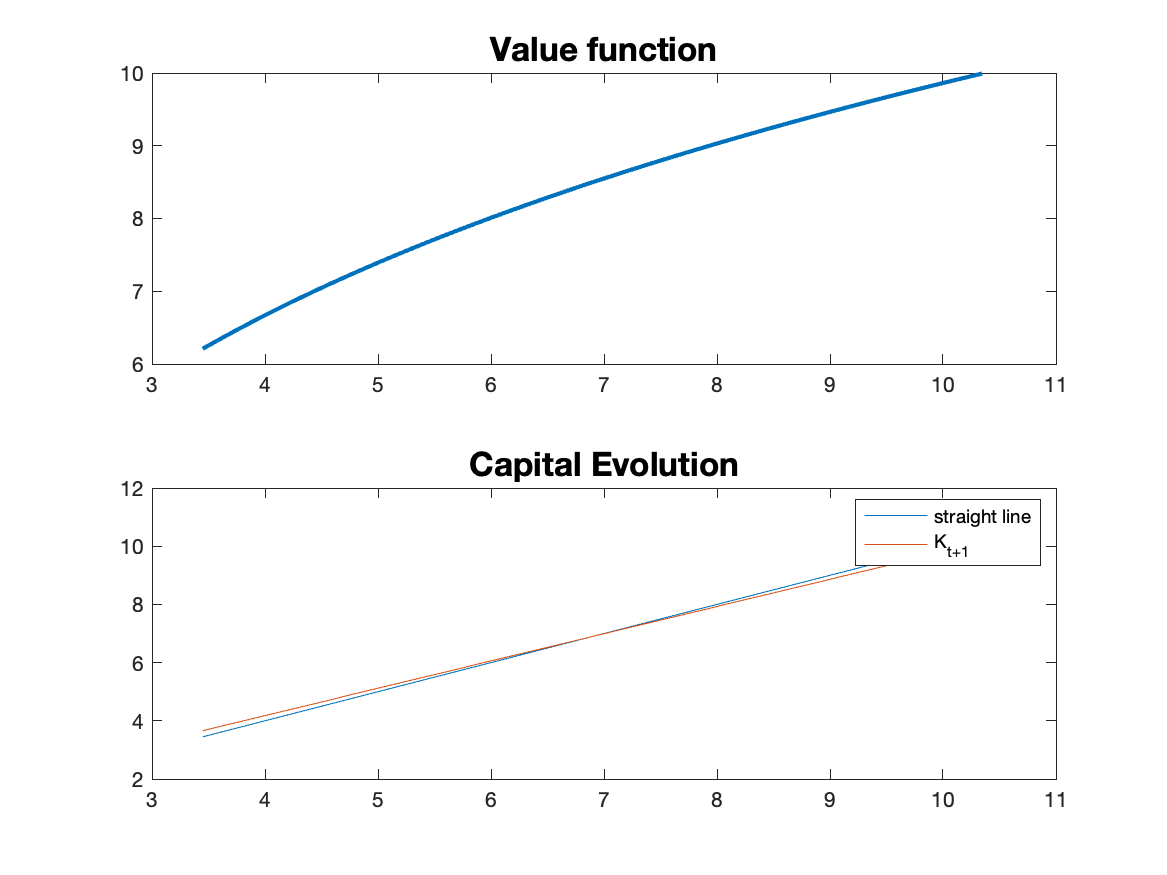
\includegraphics[width = .5\linewidth]{HW3/pics/HW3_Q2_figure.png}
       \caption{The steady state equilibrium would be stable as the $k_{t+1}$ function is above the 45 degree line before the steady state and below the 45 degree line after the steady state}
       \label{fig:HW3_2c}
   \end{figure}
   \item see above
   \item .
   \begin{figure}[H]
       \centering
       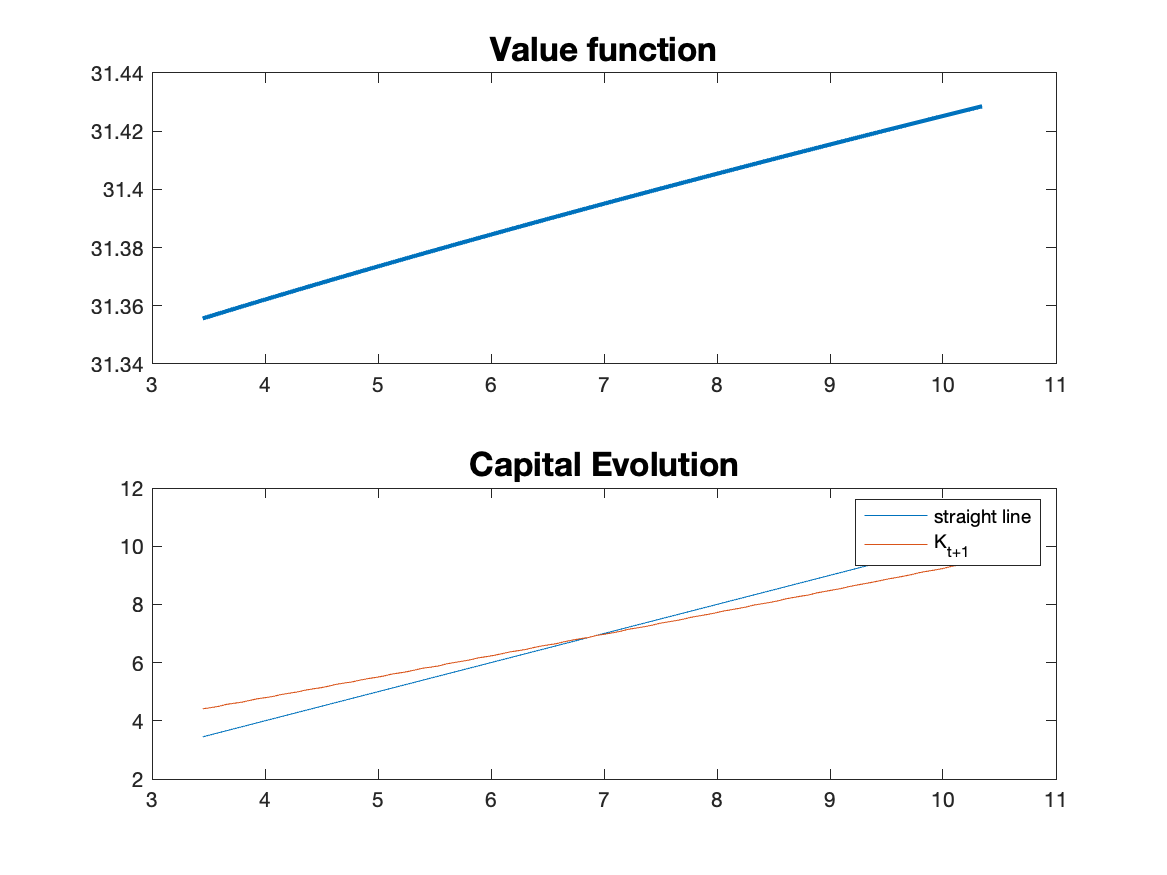
\includegraphics[width = .5\linewidth]{HW3/pics/HW3_Q2_e_figure.png}
       \caption{Similar to part c, the steady state equilibrium would be stable. The main difference is the slope of the $K_{t+1}$ line. This time the line is much more steep than the solution in part c. this is primarily due to the fact that the large endowment makes it easier for an individual to save, additionally the value function is much flatter this is because the income of production is far less important because of the large endowment}
       \label{fig:HW3_2e}
   \end{figure}
\end{enumerate}